\section{Results}
\subsection{Whole-workflow checking boosts confirmation without net repair gains}
In Study A, across three batches on the 54 official tasks (162 pairs), \texttt{v1} raises pre-edit target counterevidence from V5's 17/14/15 tasks to 27/29/28, and joint counterevidence-plus-replay from 15/11/14 to 20/23/25 (39 to 60 and 37 to 53 on all 95 tasks in R03). Yet confirmed passes tie at 75 vs 75 across 143 normal pairs (27 vs 25, 23 vs 26, 25 vs 26 per batch; seven gains, seven losses; external 29 tasks: 48 vs 47). Probing burns budget (SymPy23950 spends 11 calls before its first edit hits the cap), narrow checks pass on partial fixes (Requests7427), and unverified edits break working code (pytest7205 deletes \texttt{saferepr}).

\subsection{Stage 1: CLI invocation syntax filters out over a third of generated checks}
In Study B's final configuration (R03/R04, Table~\ref{tab:construction}), the constructor emits output in 85 of 108 realizations (up from 21/108 in R01/R02), but only 20 checks reach target behavior with a grounded expectation: 13 match the expectation and 7 expose counterevidence on a failing draft.

\begin{table}[htbp]
\centering\small
% Generated by scripts/build_v04_visuals.py from frozen v0.4 analysis.
\begin{tabular}{lr}
\toprule
Check-construction outcome & Realizations \\
\midrule
No execution output & 23 \\
Python invoked on missing \texttt{PY} file & 38 \\
Other failure before target behavior & 7 \\
Peripheral behavior only & 9 \\
Target reached; expectation insufficiently grounded & 11 \\
Grounded target behavior & 20 \\
\midrule
Total attempts & 108 \\
\bottomrule
\end{tabular}

\caption{Check-construction outcomes across 108 R03/R04 realizations (54 tasks, two seeds).}
\label{tab:construction}
\end{table}

The top failure is shell syntax rather than diagnostic logic: \textbf{38 of 108 attempts (35\%) fail with \texttt{can't open file '.../PY'}} on \texttt{python3 -B PY}. Attempting an inline heredoc (\texttt{python3 -B - << 'PY'}), the constructor omits \texttt{- <<}, so Python treats \texttt{PY} as a missing file; the rest split into 7 pre-target crashes, 9 peripheral checks, and 11 ungrounded target checks.

\subsection{Stage 2: Action substitution and silent read resets absorb saved test calls}
Stratifying the 108 R03/R04 realizations by D's grade (40 passing, 64 failing, 3 unknowns, 1 unscored; Figure~\ref{fig:actions}A), advance results on the 64 failing drafts halve replay from \textbf{46/64 (72\%) in C to 22/64 (34\%) in F} (82 to 43 overall), without adding \textbf{retained edits} (8 vs 8; 10 vs 9 overall) or \textbf{passes} (3 vs 3; two gains, two losses on 63 pairs).

\begin{figure}[htbp]
\centering
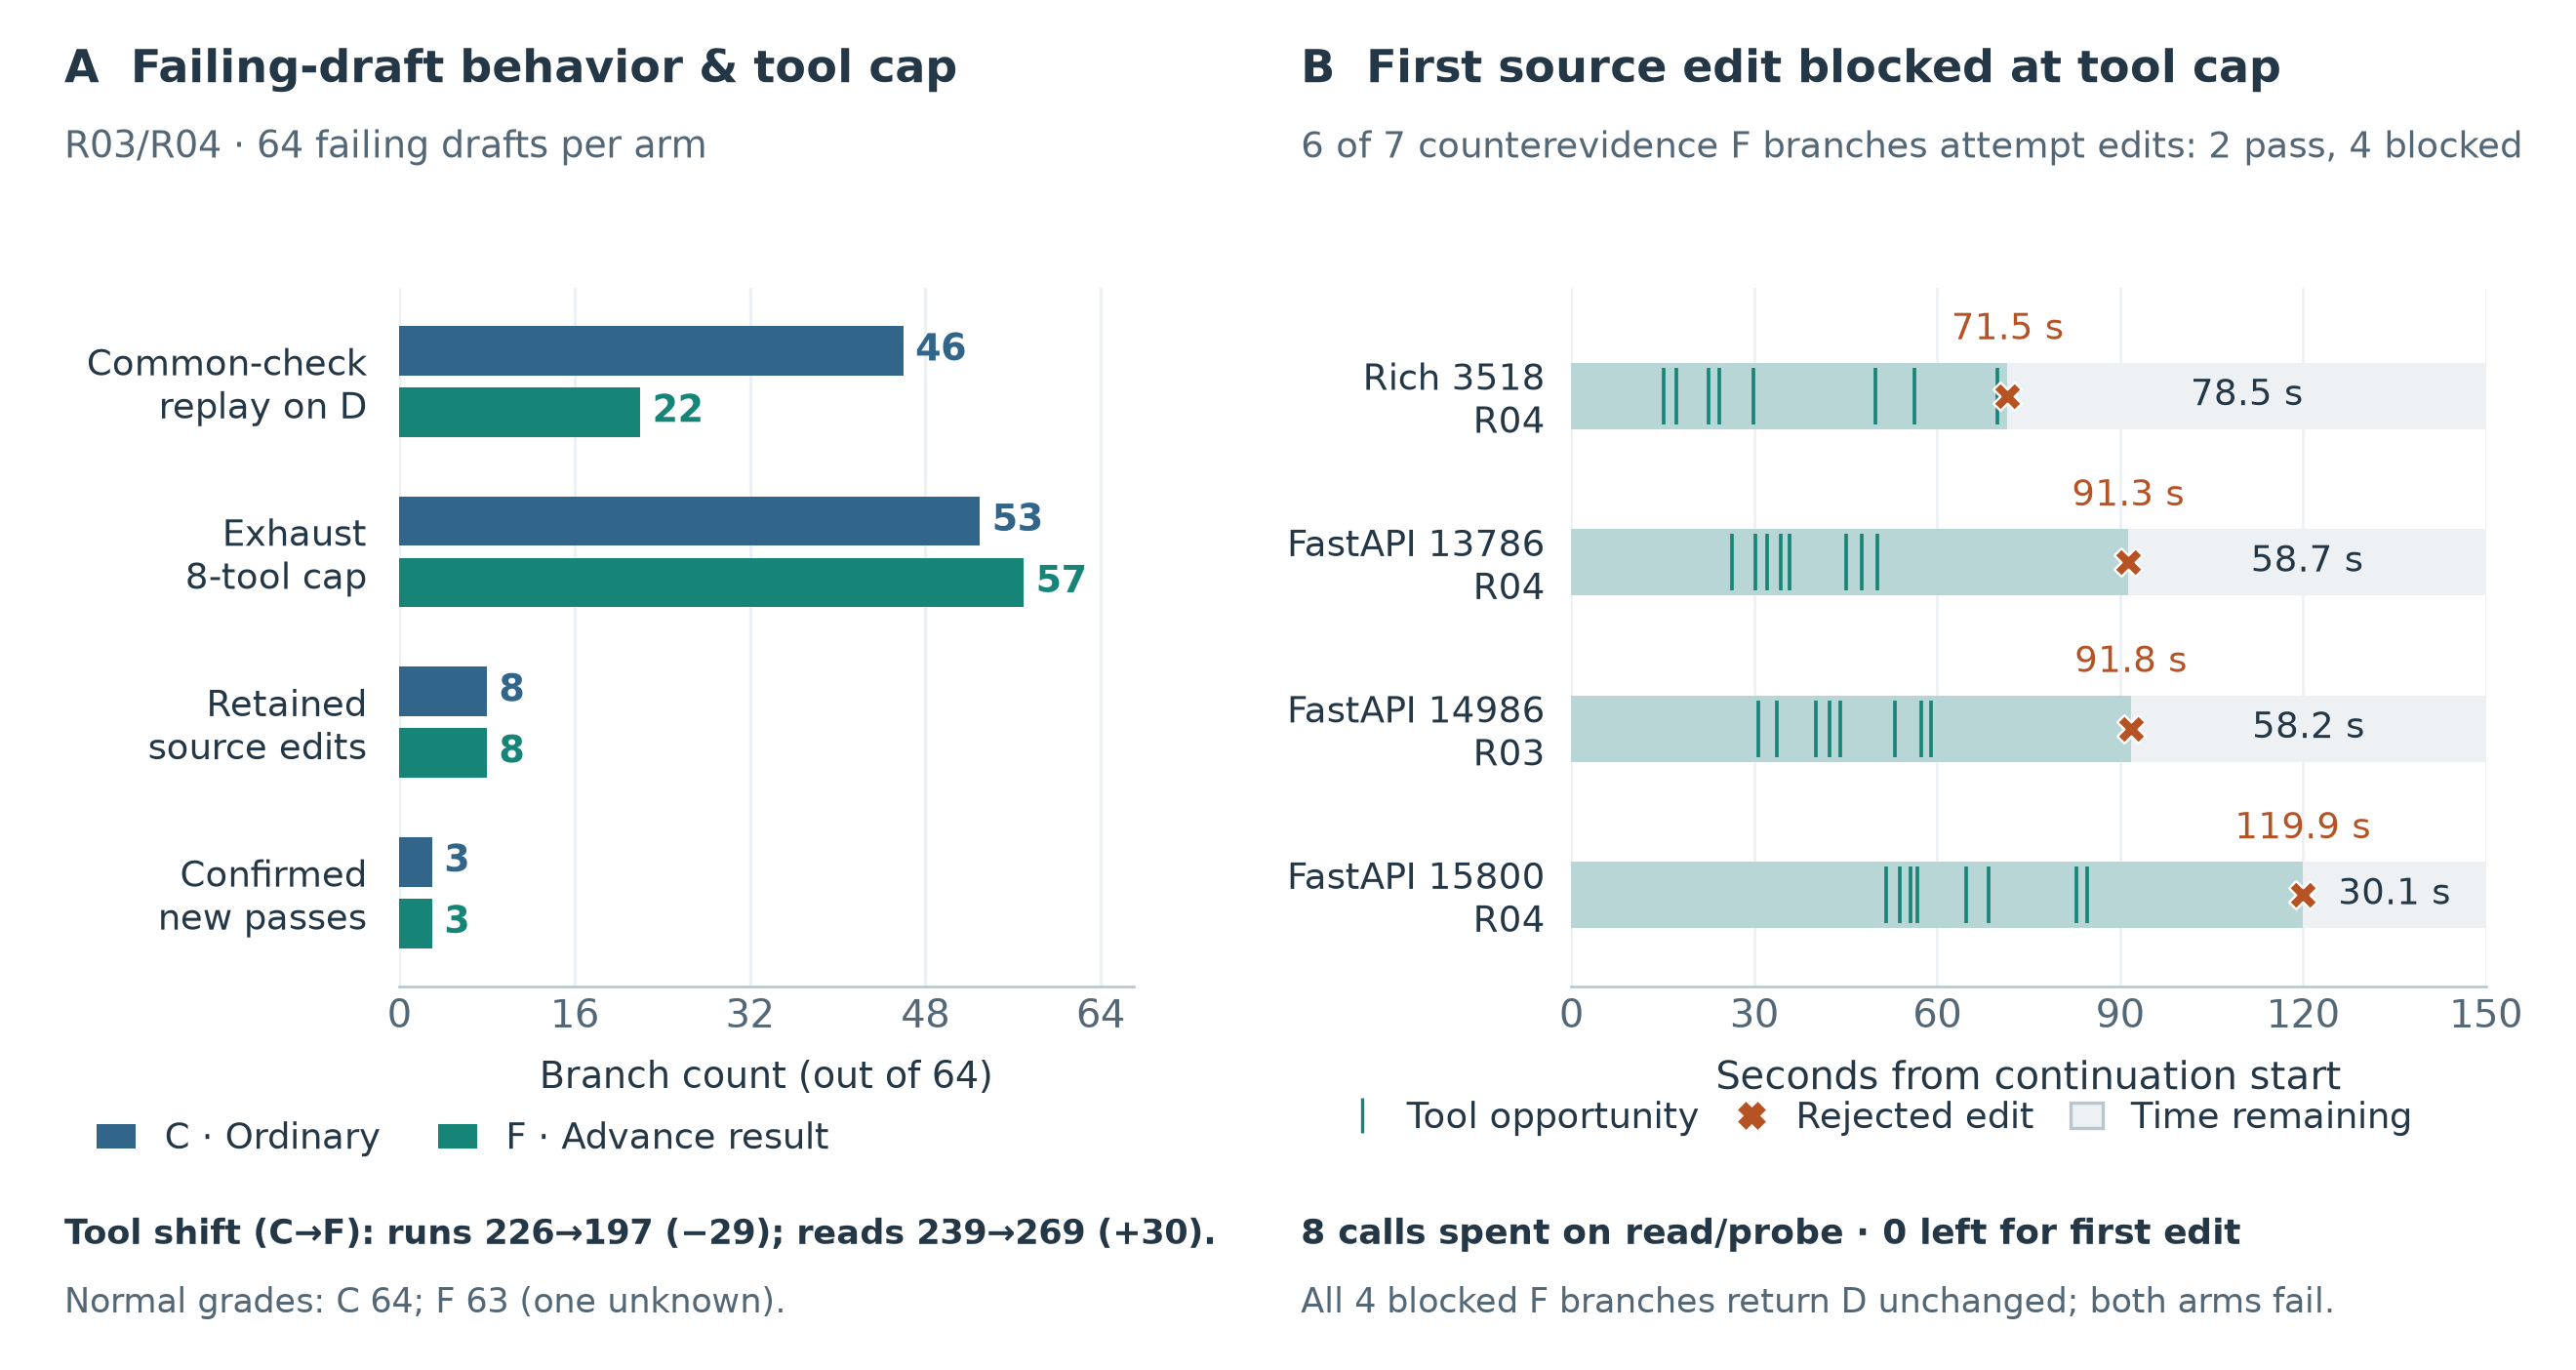
\includegraphics[width=\linewidth]{figures/feedback-and-edit-budget-v04.png}
\caption{R03/R04 failing-draft continuations and counterevidence timelines. (A) Advance results halve replay on 64 failing drafts, but agents trade command runs for file reads. (B) Four counterevidence F branches have their first edit blocked at the cap with 30--79 s left.}
\label{fig:actions}
\end{figure}

Auditing executed calls on the 64 failing drafts shows why: \textbf{agents substitute file reading for test execution}. Compared with C, F runs \textbf{29 fewer \texttt{run\_command} calls} (226 to 197) and 11 fewer \texttt{get\_status} calls (17 to 6), but adds \textbf{30 \texttt{read\_file} calls} (239 to 269; 387 to 328 and 390 to 433 overall). Moreover, \textbf{58 executed \texttt{read\_file} calls across R03/R04 (25 C, 33 F; 24 on failing drafts)} pass a malformed optional key (\texttt{"start\_line"": "151"}); because \texttt{start\_line} is optional, the tool ignores it and \textbf{silently resets to lines 1--150 in 56 of 58 calls} (24 C, 32 F). Sharing one eight-call pool means \textbf{89\% of F branches on failing drafts (57/64) and 83\% of C branches (53/64) hit \texttt{BudgetExceeded}} (\href{supplement/continuation-process-v04.md}{process table}).

\begin{table}[htbp]
\centering\small
% Generated by scripts/build_v04_visuals.py from frozen v0.4 analysis.
\begin{tabular}{lrrrrrrrr}
\toprule
 & & \multicolumn{2}{c}{Replay} & \multicolumn{2}{c}{Retained edits} & & \multicolumn{2}{c}{F vs C} \\
\cmidrule(lr){3-4}\cmidrule(lr){5-6}\cmidrule(lr){8-9}
Common result & N & C & F & C & F & Pairs & Gains & Losses \\
\midrule
Grounded target & 20 & 20 & 4 & 1 & 3 & 20 & 1 & 0 \\
Other output & 65 & 62 & 39 & 4 & 5 & 62 & 1 & 1 \\
No output & 23 & 0 & 0 & 5 & 1 & 21 & 0 & 2 \\
\bottomrule
\end{tabular}

\caption{R03/R04 continuations by check quality. Replay counts pre-edit runs on D; edits count retained diffs; gains/losses compare F against C.}
\label{tab:strata}
\end{table}

Stratifying by check quality (Table~\ref{tab:strata}) links Stage 1 to Stage 2. In \emph{Other output} (65 realizations, including the 38 \texttt{python3 -B PY} crashes), F receives a shell error, forcing \textbf{60\% (39/65)} of F branches to re-run or repair the check. In \emph{Grounded target} (20 realizations: 10 passing D, 10 failing D), F replay drops \textbf{80\% (20/20 to 4/20)}, call-0 \texttt{read\_file} starts jump from \textbf{6/20 (30\%) to 16/20 (80\%)}, and edit-attempting branches double from \textbf{4/20 to 8/20}---yet 4 of 8 hit \texttt{BudgetExceeded}, leaving 3 retained edits vs 1 in C (+1 pass).

\subsection{Stages 3 and 4: The last-centimeter edit wall, delimiter corruption, and draft regression}
The seven R03/R04 realizations with grounded counterevidence on a failing draft (eight across all batches, adding FastAPI13537/R02) expose Stages 3 and 4. Whereas 4 of 7 C branches attempt an edit, \textbf{6 of 7 F branches (7 of 8 overall) issue a concrete \texttt{edit\_file} call} across four outcomes:

\textbf{1. Landed within cap (2/7 F in R03/R04, 3/8 overall; 100\% pass).} Every counterevidence branch executing \texttt{edit\_file} within the cap passes: Requests6592/R03 in both arms (\texttt{too\_early} 425 alias at call 2), Rich3067/R03 F (regex fix at call 6 after two schema retries, verified at call 7), and FastAPI13537/R02 F (\texttt{processed\_keys} in \texttt{\_extract\_form\_body} at call 6, verified at call 7).

\textbf{2. Exact, uniquely matching fixes preempted by one slot (2/7 F: Rich3518/R04 and FastAPI13786/R04, plus Rich3518/R04 C).} Static verification against D shows both formulate an \texttt{edit\_file} with an \textbf{exact unique match (\texttt{occurrences = 1})} fixing the failing assertion. In Rich3518/R04 (\texttt{Column.highlight} not inherited from \texttt{Table}), F (event 8, 71.5 s, 78.5 s left) and C (event 9, 44.1 s) emit the identical fix at line 456 of \texttt{rich/table.py} (\texttt{column = Column(\_index=index, highlight=self.highlight)})---after F lost one slot at event 1 (\texttt{"start\_line"": "151"}) and C lost two at events 4--5 to silent line-1 resets. In FastAPI13786/R04 (\texttt{WWW-Authenticate} formatting \texttt{APIKeyIn.query} instead of \texttt{"query"}), F verifies the enum bug via \texttt{python3 -c}, hits \texttt{BudgetExceeded} on \texttt{grep} at event 8, and at event 9 (91.3 s, 58.7 s left) emits \texttt{self.model.in\_.value} on \texttt{fastapi/security/api\_key.py}.

\textbf{3. Multi-part tasks cut off mid-localization (2/7 F: FastAPI14986/R03 and FastAPI15800/R04, plus FastAPI15800/R04 C).} Both require two-file edits (\texttt{applications.py} plus \texttt{docs.py} or \texttt{routing.py}). When \texttt{BudgetExceeded} interrupts localization at event 8 (Figure~\ref{fig:actions}B), the model emits a truncated edit on \texttt{applications.py} at event 9: FastAPI14986/R03 F emits a bare \texttt{old\_string} (\texttt{"] = True,"} to \texttt{"] = False,"}) leaving \texttt{docs.py} unedited, while FastAPI15800/R04 F and C overwrite an anchor header (\texttt{def include\_router(} or \texttt{def \_\_init\_\_(}) to insert \texttt{def frontend(}.

\textbf{4. Cut off at target-file entry (1/7 F: FastAPI15589/R04).} F spends six calls reading \texttt{fastapi/params.py} (with a silent \texttt{"start\_line"": "600"} reset at event 1), locates \texttt{convert\_underscores} in \texttt{fastapi/dependencies/utils.py} via \texttt{grep} at events 6--7, and has its first \texttt{read\_file} on \texttt{utils.py} (lines 750--850) blocked by \texttt{BudgetExceeded} at event 8 (46.7 s, 103.3 s left).

\textbf{Stage 4A: Delimiter corruption and retry loops (93 calls, 11 branches).} Across R03/R04, C and F incur \textbf{45 and 48 (93 total, all on failing drafts) \texttt{edit\_file} rejections} for missing \texttt{old\_string} across \textbf{11 branches} (6 C, 5 F; mean 8.5/branch, peaking at 17 in Rich3067/R03 C and 24 in Rich3718/R04 F). Raw arguments show \textbf{in 93 of 93 calls (100\%), the model emitted \texttt{old\_string:}}: when editing code with quotes, colons, or regexes, delimiter corruption fuses \texttt{,old\_string:} into \texttt{new\_string}, and in \textbf{82 of 93 (88\%)} splits target code on colons and commas into bogus keys. Because schema errors do not decrement the cap and report only \texttt{old\_string} as missing, the model repeats the corrupted call.

\textbf{Stage 4B: Continuation regression.} Across all batches, 29 of 432 patches retain executable diffs over D (plus 3 docstrings and 1 restored edit), yet \textbf{4 of 29 delete working logic}. Among 40 passing drafts in R03/R04, C retains 40 passes and F retains 39: in Requests7433/R03, F deletes D's passing \texttt{hasattr(data, "\_\_iter\_\_")} fallback and hits its cap before restoring it; in Rich3067/R04, F corrupts \texttt{highlighter.py} via \texttt{sed} and reverts to D while C passes.

\FloatBarrier
